\section{Experiments} \label{sec:experiment}
In this section, we measure the overall performance of the optimized 
HLS based BFS accelerator on Alpha Data ADM-PCIE-7v3 using a set of 
representative graphs. Then we compare the resulting accelerator to 
both a baseline design which has best-effort HLS optimization applied to 
native BFS code and existing FPGA based BFS acceleration work. Then we evaluate 
the major design optimization methods including pipelining, redundancy removal,  
caching and data path duplication proposed in this work. 

\subsection{Experiment Setup}
The graph benchmark used in this work includes three real-world graphs and 
two synthetic graphs generated using R-MAT model \cite{chakrabarti2004rmat} 
as listed in Table \ref{tab:graph}. The real-world graphs are from social network \cite{yang2012defining, 
leskovec2009community, takac2012data} while the R-MAT graphs are generated 
using the Graph 500 benchmark parameters ($A=0.59, B=0.19, C=0.19$). To make the 
presentation easier, the five benchmark graphs are shorted as Youtube, 
LJ, Pokec, R-MAT\uppercase\expandafter{\romannumeral1}, 
R-MAT\uppercase\expandafter{\romannumeral2} respectively. We refer 
to an R-MAT graph with scale $S$ ($2^{S}$ nodes) and edge factor $E$ ($E\times 2^{S}$). 
In order to avoid trivial search, we only choose vertices from the largest 
connected component as the BFS starting point.

\begin{table}
    \centering
  \caption{Graph Benchmark}
  \label{tab:graph}
  \begin{tabular}{cccc}
    \toprule
      Name & \# of vertex & \# of edge & Type \\
    \midrule
      Youtube \cite{yang2012defining} & 1157828 & 2987624 & Undirectional \\
      LJ \cite{leskovec2009community} & 4847571 & 68993773 & Directional \\
      Pokec \cite{takac2012data} & 1632804 & 30622564 & Directional \\
      R-MAT\uppercase\expandafter{\romannumeral1} & 524288 & 16777216 & Directional \\
      R-MAT\uppercase\expandafter{\romannumeral2} & 2097152 & 67108864 & Directional \\
  \bottomrule
\end{tabular}
\end{table}

\subsection{Performance comparison}
We use the million traverse per second (MTEPS) as 
the performance metric. The performance of the proposed BFS 
accelerator on the graph benchmark is 
presented in Table \ref{tab:performance-summary}. 
It gets up to 82.16 MTEPS on the R-MAT\uppercase\expandafter{\romannumeral1} graph and achieves 
38.83 MTEPS on average. When compared to a baseline HLS based 
BFS accelerator, the proposed design shows 24.7X to 77.5X performance 
speedup on the five benchmark graphs. Note that the baseline HLS design 
refers to a native C/C++ based BFS implementation 
with best effort HLS pragma optimization but no modification of the source code.
With the comparison, it is clear that straightforward HLS optimizations 
are far from sufficient and dedicated high level optimizations are critical to 
the performance of the resulting BFS accelerator.
\begin{table}
    \centering
  \caption{Performance summary}
  \label{tab:performance-summary}
  \begin{tabular}{cccccc}
    \toprule
      Benchmark & Youtube & LJ & Pokec & RMAT\uppercase\expandafter{\romannumeral1} & RMAT\uppercase\expandafter{\romannumeral2} \\
    \midrule
      MTEPS & 14.35 & 28.05 & 36.94 & 82.16 & 32.67 \\
      Speedup & 77.50 & 36.82 & 38.83 & 62.18 & 24.70 \\
  \bottomrule
\end{tabular}
\end{table}

On top of the comparison to the baseline HLS design, we also compare 
this work to a set of existing BFS accelerators on FPGAs. As the platforms 
and graph benchmark used in these work are mostly different, it is 
difficult to make a fair end-to-end comparison. Hereby, we add
MTEPS per unit bandwidth (MTEPSPB) as an additional performance metric showing the 
potential of the BFS accelerators on different hardware platforms. 
A rough comparison result is listed in Table \ref{tab:compare}. It can be found that the HLS 
based BFS accelerator proposed in this work achieves around 35\% of the 
performance in \cite{zhang2017boosting}. Nevertheless, the memory bandwidth 
is much lower compared to that in \cite{zhang2017boosting} and the per bandwidth 
MTEPS in this work outperforms especially on the R-MAT graphs. Compared to the 
general graph processing framework based BFS accelerator in \cite{dai2016fpgp} and 
\cite{nurvitadhi2014graphgen}, this work shows competitive per bandwidth MTEPS on either 
the R-MAT graph or the graph benchmark. When compared to design on high-end 
FPGA computing system, the performance is still much lower while the per bandwidth 
performance is around 25\% of the highly optimized handcraft design and 
the HLS based design gains the software-like features.

\begin{table}
  \caption{FPGA based BFS accelerator comparison}
  \label{tab:compare}
    \setlength{\tabcolsep}{4pt} % Default value: 6pt
    %\renewcommand{\arraystretch}{1.5} % Default value: 1
  \begin{tabular}{cccccc}
    \toprule
      Work & Platform & Graph & MTEPS & BW(GB/s) & MTEPSPB \\
    \midrule
      \cite{betkaoui2012reconfigurable} & Convey HC-2 & R-MAT & 1600 & 80  & 20 \\
      \cite{attia2014cygraph} & Convey HC-2 & R-MAT    & 1900 & 80  & 24.4 \\
      \cite{zhang2017boosting} & Micro-AC510       & R-MAT  & 166.2  & 60  & 2.8 \\
      \cite{nurvitadhi2014graphgen} & VC707 Kit & Twitter & 148.6 & 6.4 & 9.9 \\
      \cite{dai2016fpgp}  & VC707 Kit & Twitter & 12  & 6.4 & 1.9 \\
      this work & ADM-PCIe-7v3 & R-MAT & 57.41 & 10.8 & 5.3 \\
      this work & ADM-PCIE-7v3 & Graph in Table \ref{tab:graph} & 38.8 & 10.8 & 3.6 \\
  \bottomrule
\end{tabular}
\end{table}

\subsection{Pipelining Optimization}
We can convert the BFS algorithm with nested loops to 
a stream design with six pipeline stages as illustrated in Algorithm \ref{alg:bfs-stream}. 
To explore pipelining influence, we build a series of implementations 
with different pipelining configurations. By dividing f5 into two dependent parts i.e. f5.1 
and f5.2, we build a seven-stage pipelined BFS accelerator. By combing the 
pipelining stages, we also create accelerators with less pipelining stages. 
The different pipeline configurations are listed in Figure \ref{fig:pipeline-config} 
and the performance comparison is presented in Figure \ref{fig:pipeline-performance}.

According to the experiments, we find that more pipeline stages are typically beneficial to 
the final performance. Particularly, we observe that the resulting BFS accelerator 
performance has significant improvement when the number of pipeline stages 
jumps from 1 to 2 and from 5 to 6. Thus we try to keep the critical pipeline stages 
and further construct new pipeline configurations i.e. c8 and c9. 
The performance, however, is not improved as expected. The comparison also indicates 
that the internal pipeline stages are also important to the 
overall BFS accelerator performance. It is just that they are dependent 
and any one of the sub function that fails to be pipelined will 
stall the overall pipeline and affect the final performance. 

\begin{figure}
\center{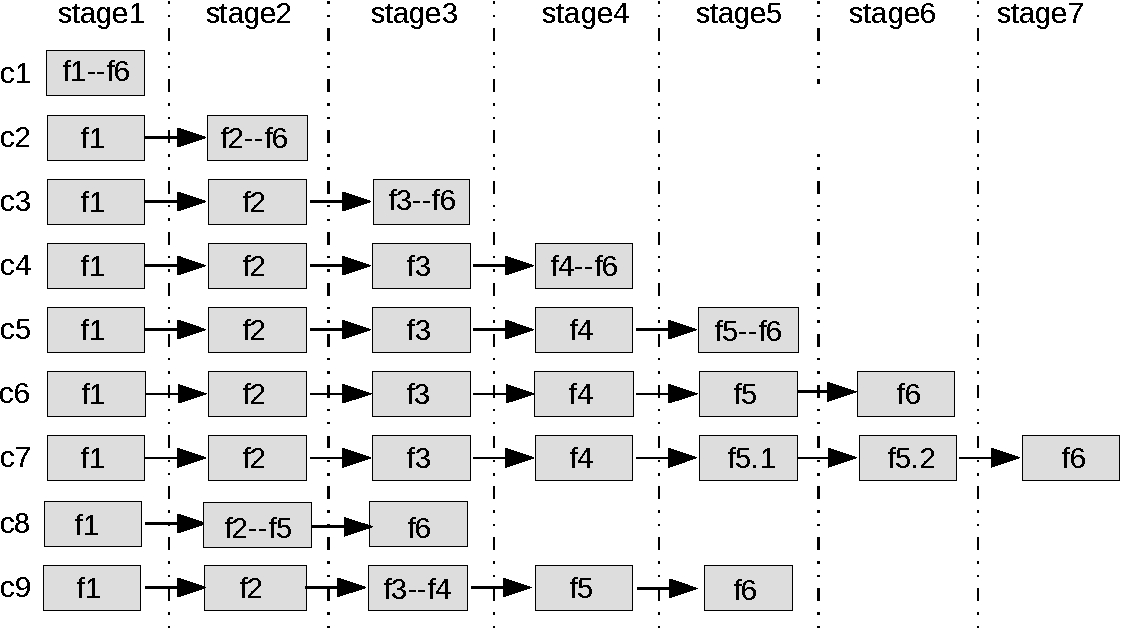
\includegraphics[width=0.95\linewidth]{pipeline-config}}
    \caption{Pipeline configurations with various combinations.}
\label{fig:pipeline-config}
\end{figure}

\begin{figure}
\center{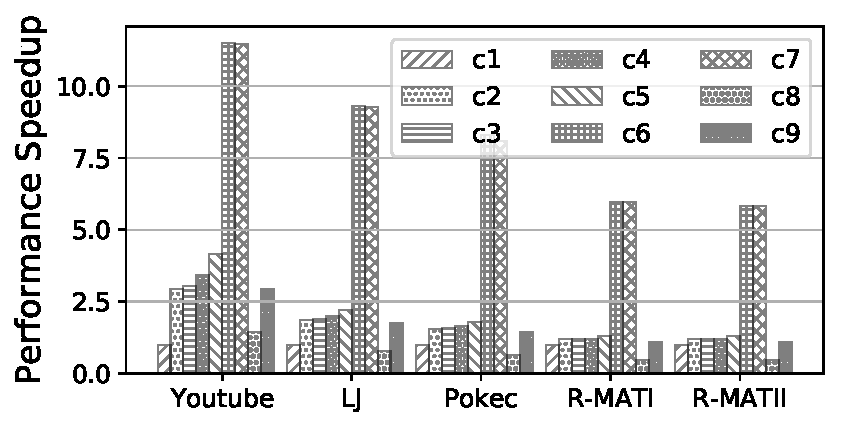
\includegraphics[width=0.95\linewidth]{pipeline-performance}}
    \caption{Performance speedup over a baseline design c1.}
\label{fig:pipeline-performance}
\end{figure}

Table \ref{tab:hash-resource} shows the FPGA resource consumption of the different 
pipeline configurations. It can be found that deeper pipelined implementations typically 
consume more hardware resources including LUT and FF for constructing the 
computing logic and the buffers between the pipeline stages. The RAM blocks in the design 
are used for buffering data for global memory access and each global memory port requires 
two BRAM\_18K blocks by default. Hereby, it is not relevant to the pipeline depth but relevant to 
the amount of global memory ports. 
Since there is almost no computing involved in the BFS accelerator design, only a fractional 
FPGA resources are consumed.

According to the performance and resource consumption experiments, we find that 
c6 achieves near optimal performance with reasonable hardware resource overhead.
Therefore, it is taken as the optimized pipelining setup in the following experiments.

\begin{table}
  \caption{FPGA resource consumption with different pipelining configurations}
  \label{tab:hash-resource}
  %\setlength{\tabcolsep}{4pt} % Default value: 6pt
  %\renewcommand{\arraystretch}{1.5} % Default value: 1
    \centering
  \begin{tabular}{ccccccc}
    \toprule
      Config. & FF & \% & LUT & \% & RAMB18K & \% \\
    \midrule
      c1 & 3581 & $\sim$0 & 4289 & $\sim$0 & 8  & $\sim$0 \\
      c2 & 4121 & $\sim$0 & 5416 & $\sim$1 & 10 & $\sim$0 \\
      c3 & 4208 & $\sim$0 & 5746 & $\sim$1 & 10 & $\sim$0 \\
      c4 & 4494 & $\sim$0 & 6675 & $\sim$1 & 10 & $\sim$0 \\
      c5 & 4551 & $\sim$0 & 7022 & $\sim$1 & 10 & $\sim$0 \\
      c6 & 5546 & $\sim$0 & 8126 & $\sim$1 & 12 & $\sim$0 \\
      c7 & 5853 & $\sim$0 & 8154 & $\sim$1 & 12 & $\sim$0 \\
      c8 & 5113 & $\sim$0 & 7152 & $\sim$1 & 12 & $\sim$0 \\
      c9 & 5408 & $\sim$0 & 7843 & $\sim$1 & 12 & $\sim$0 \\
  \bottomrule
\end{tabular}
\end{table}

\subsection{Memory access optimization}
We have implemented a series of memory optimizations including 
redundancy removal, prefetching and caching on top of the pipelined 
BFS accelerator. These optimizations are tuned 
based on corresponding metrics obtained through software emulation. 

\subsubsection{Redundancy removal analysis} 
To squeeze the redundancy in the output stream of f4, we create a hash table based 
filter as presented in Section \ref{sec:bfs-opt} and insert it between f4 and f5. 
The hash table size affects the redundancy removal rate and the performance eventually.
To decide the hash table size rapidly, we thus analyze the correlation 
between the hash table size and the redundancy removal rate with 
fast software emulation. 

Figure \ref{fig:hash-redundancy} shows the 
redundancy removal rate of different size of hash tables. Basically larger hash table 
can improve the redundancy removal rate in general, but the improvement gets trivial 
when the hash table size is large enough. In this work, we keep doubling the hash table and stop 
until the hash table hit rate (redundancy removal rate) improvement starts to slow down significantly. 
With this metric, the final hash table setup of the different graphs is given in 
Table \ref{tab:hash-size}.

\begin{figure}
\center{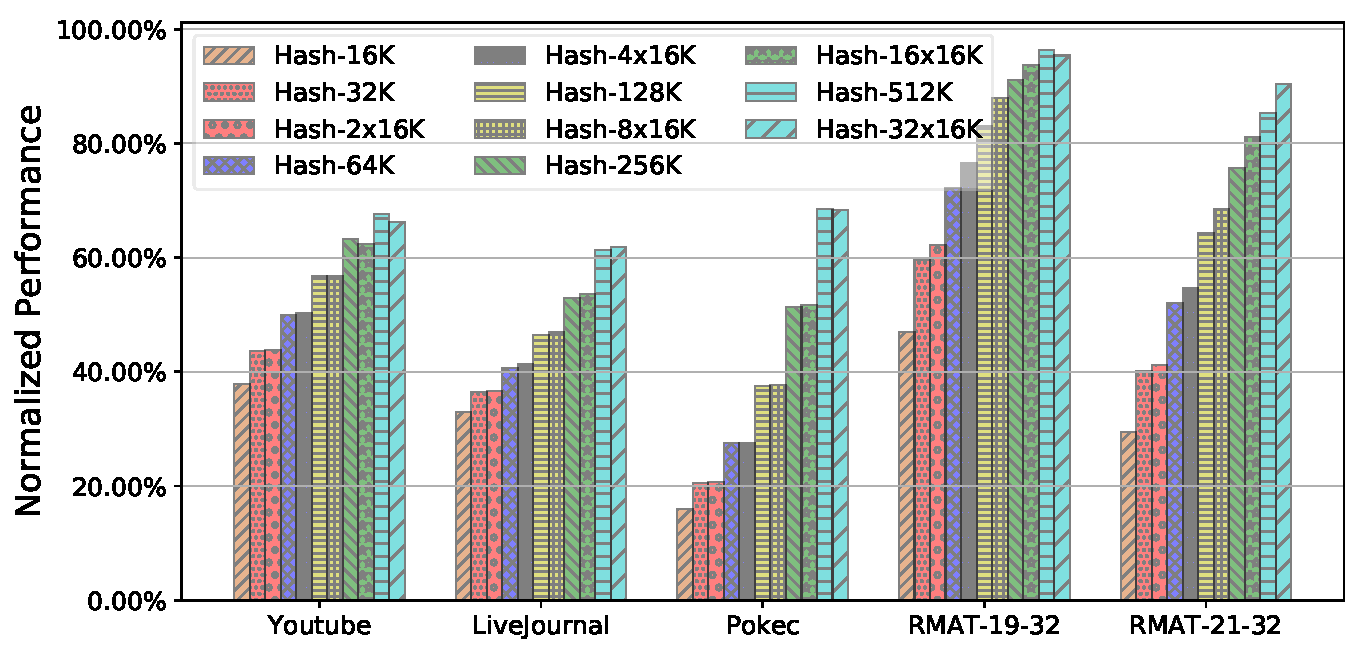
\includegraphics[width=0.95\linewidth]{hash-redundancy}}
    \caption{Correlation between redundancy neighbor vertices removal rate and the hash table size. 
    The redundancy removal rate varies on the different graphs. The optimized hash table size also 
    differs.}
\label{fig:hash-redundancy}
\end{figure}

\begin{table}
    \centering
  \caption{Hash table size setup}
  \label{tab:hash-size}
  \begin{tabular}{cccccc}
    \toprule
      benchmark & Youtube & LJ & Pokec & R-MAT\uppercase\expandafter{\romannumeral1} 
      & R-MAT\uppercase\expandafter{\romannumeral2} \\
    \midrule
      size (K entries) & 256 & 2048 & 1024 & 512 & 1024 \\
  \bottomrule
\end{tabular}
\end{table}

\subsubsection{Cache analysis}
As described in Section \ref{sec:bfs-opt}, we have 
cache structures for random \textit{depth} reading 
and writing in f5 and f6 respectively. 
Similar to the hash table size setup, we decide the 
cache size based on the cache hit rate analysis while the cache 
hit rate can be obtained through software emulation of the HLS design. 

Figure \ref{fig:cache-hit} shows the correlation 
between the cache size and the resulting cache 
hit rate. According to the experiment in the figure,  
the cache size influence varies dramatically on different graphs. 
Particularly, we find that R-MAT\uppercase\expandafter{\romannumeral1} 
reaches nearly optimal hit rate when the cache size is 8K$\times$64B i.e. 
8K entries with 64B cache line. For the Youtube and Pokec graphs, cache hit 
rate is satisfactory when the cache size goes up to 
16K$\times$64B. Live Journal graph requires much higher cache size and 
64K$\times$64B cache is an optimized setup. However, it exceeds the 
on-chip RAM blocks on the target FPGA board. As a result, we set it 
to be 32K$\times$64B in this work.

\begin{figure}
\center{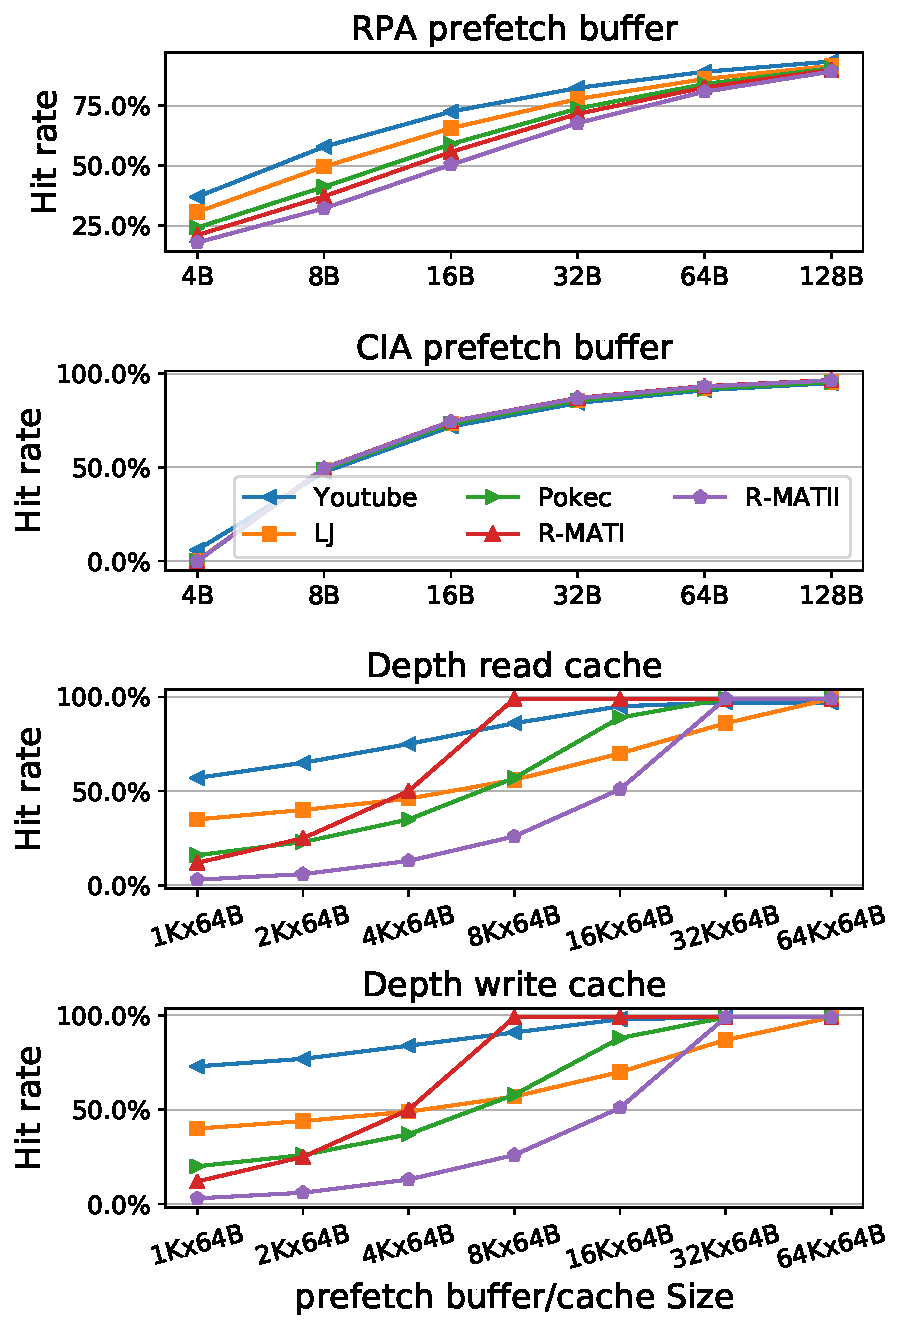
\includegraphics[width=0.95\linewidth]{cache-hit}}
    \caption{Cache configurations have significant influence on the cache hit rate.
    The influence varies on different graph data set, but the trend is similar.}
\label{fig:cache-hit}
\end{figure}

\begin{table}
    \centering
  \caption{Cache size setup}
  \label{tab:hash-size}
  \begin{tabular}{cccccc}
    \toprule
      benchmark & Youtube & LJ & Pokec & R-MAT\uppercase\expandafter{\romannumeral1}
      & R-MAT\uppercase\expandafter{\romannumeral2} \\
    \midrule
      size (K entries) & 16 & 32 & 16 & 8 & 32 \\
  \bottomrule
\end{tabular}
\end{table}

\subsubsection{Prefetch buffer analysis}
We explore the correlation between prefetch buffer size and  
buffer hit rate through the software emulation as well. The result is 
shown in Figure \ref{fig:prefetch-hit}. Unlike the cache in BFS accelerator,  
the influence of the prefetch buffer varies slightly on different 
graph benchmark and 64B prefetch size achieves satisfactory 
hit rate. 64B is also the optimized global memory access data width 
and a single read operation completes the prefetch at buffer miss simplifying the 
HLS initialization interval optimization. With these reasons, 
we choose 64B as the prefetch buffer size for all the different graphs.
The prefetch buffer consumes negligible hardware resources, so the resource overhead 
is skipped to save the space.

\begin{figure}
\center{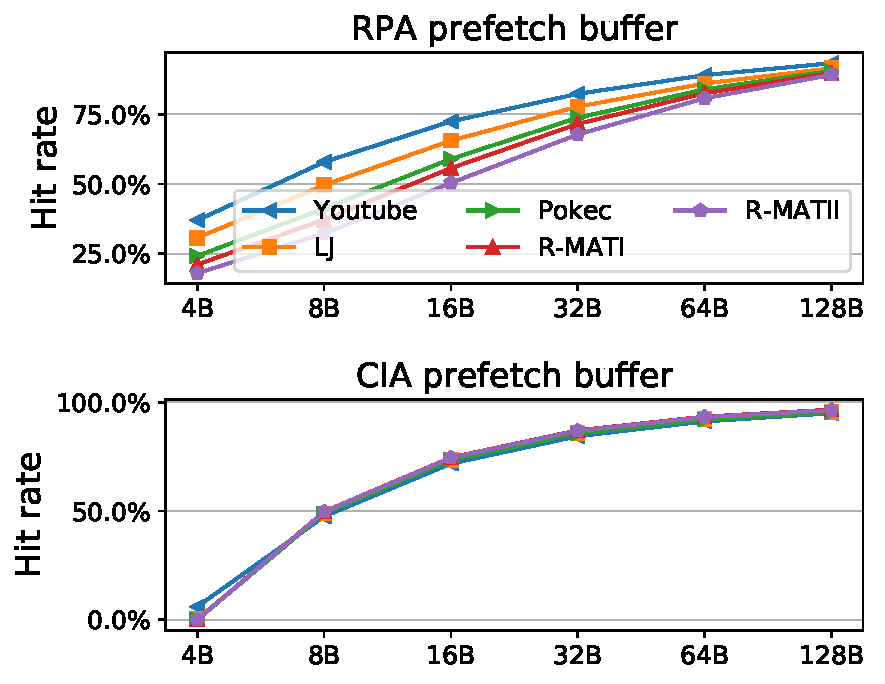
\includegraphics[width=0.95\linewidth]{prefetch-hit}}
    \caption{A small prefetch buffer can already achieve high hit rate.
    Particularly the prefetch buffer size influence on different graph 
    data set is similar.}
\label{fig:prefetch-hit}
\end{figure}

\subsubsection{Parameters of the memory optimizations}
According to the experiments, both hash table and cache require large amount of 
block RAMs. As a result, optimized setup can't be fulfilled at the same time.
Considering that cache can also avoid redundant memory access and 
cache hit rate is more sensitive to the cache size, we opt to 
provide block RAMs to cache first while leaving the rest for hash table. Prefetch 
buffer is much smaller compared to cache and hash table, so we set prefetch buffer 
to be 64B directly. With this strategy, the design parameter configurations 
of the memory optimization strategies are summarized and presented in 
Table \ref{tab:parameter-setup}. The hash tables for LJ and R-MATII 
as highlighted in the table are shrunk to fit for the on-chip memory constraints. 
Note that the \textit{depth} read and write cache 
are set to be the same and the cache size in the table refers to the capacity of 
one cache size.

\begin{table}
  \caption{Memory optimization parameter setup}
  \label{tab:parameter-setup}
  %\setlength{\tabcolsep}{4pt} % Default value: 6pt
  %\renewcommand{\arraystretch}{1.5} % Default value: 1
    \centering
  \begin{tabular}{ccccccc}
    \toprule
      Benchmark & Hash Table & Cache Size & Prefetch Buffer \\
    \midrule
      Youtube  & 256K  & 16K $\times$ 64B & 64B \\
      LJ       & \textbf{512K} & 32K $\times$ 64B & 64B \\
      Pokec    & 1024K & 16K $\times$ 64B & 64B \\
      R-MATI   & 512K  & 8K $\times$  64B & 64B \\
      R-MATII  & \textbf{512K} & 32K $\times$ 64B & 64B \\
  \bottomrule
\end{tabular}
\end{table}

The corresponding FPGA resource consumption is presented in Table \ref{tab:mem-resource}. 
FF and LUT consumption don't change much with the different 
design configurations and they take up only a small portion 
of the total FPGA resources. Block RAMs turns out to be the major 
resource bottleneck, and it leads to the adoption of sub optimal 
design configurations.

\begin{table}
  \caption{FPGA resource consumption}
  \label{tab:mem-resource}
  %\setlength{\tabcolsep}{4pt} % Default value: 6pt
  %\renewcommand{\arraystretch}{1.5} % Default value: 1
    \centering
  \begin{tabular}{ccccccc}
    \toprule
      Config. & FF & \% & LUT & \% & RAMB18K & \% \\
    \midrule
      Youtube  & 65244 & 7 & 108810 & 25 & 1515  & 51 \\
      LJ       & 65266 & 7 & 108829 & 25 & 2784  & 94 \\
      Pokec    & 65262 & 7 & 108812 & 25 & 2155 & 73 \\
      R-MATI   & 65244 & 7 & 108808 & 25 & 1217 & 41 \\
      R-MATII  & 65266 & 7 & 108829 & 25 & 2784 & 94 \\
  \bottomrule
\end{tabular}
\end{table}

\subsection{General HLS optimizations}
There are many HLS optimization techniques that can be applied to the 
general high level designs for better performance. We mainly explore the 
data path replication strategies in this sub section. The rest of the 
optimization techniques such as data width extension, loop unrolling, 
and loop pipelining are already well documented in Xilinx HLS user guide \cite{ug902}. 
We just adopt them as necessary and will not dwell in this paper. 

As mentioned in Section \ref{sec:bfs-opt}, we have two data path 
duplication strategies i.e. a straightforward duplication strategy and 
an optimized duplication strategy. To compare the two strategies, we analyze the percentage 
of frontier vertices that go through each duplicated data path in each BFS iteration. 
This frontier distribution over the data paths can be obtained through fast software emulation.
To make the figure clear, we just put the frontier distribution of LJ in Figure \ref{fig:load-balance}. 
It can be seen that the frontier distribution varies in a large 
range in most BFS iterations of all graphs, while the optimized data path duplication strategy 
addresses the problem efficiently. Note that sim\_4lanes represents the straightforward 
data path duplication with 4 lanes. Similarly, opt\_4lanes stands for 
the optimized data path duplication with 4 lanes.

\begin{figure}
\center{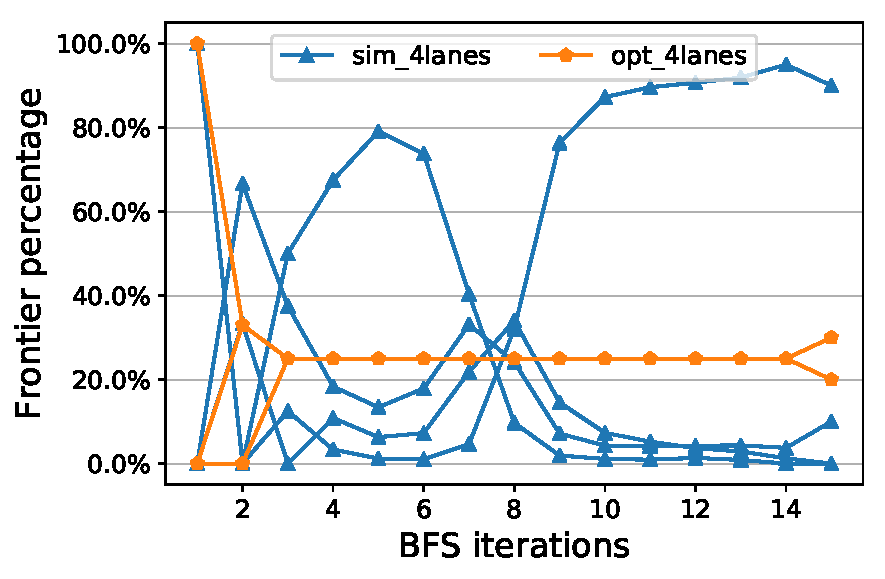
\includegraphics[width=0.95\linewidth]{load-balance}}
    \caption{Workload distribution on each data path. We take the percentage of 
    the frontier vertices in each BFS iteration as the workload.}
\label{fig:load-balance}
\end{figure}

SDAccel allows at most 16 global memory ports in a hardware thread while 
the amount of global memory ports increases when the data path is duplicated.
Six global memory ports are needed in the basic six-stage pipelined design.
Using the straightforward data path duplication, the accelerator allows 
at most 2 lanes of data paths. Using the optimized data path duplication strategy 
proposed in Sec \ref{sec:bfs-opt}, 4 lanes of data paths can be implemented.

According to the above analysis, we can confirm that the optimized data path duplication 
strategy has clear advantage on load balance and allows more 
parallel data paths in the accelerator. Hereby, it is adopted in this work.
When the data path duplication strategy is decided, the cache size and hash 
table size must be adjusted accordingly to fit for the total block ram resource 
constraint. Here we divide the hash table and depth read cache into each data 
path equally. Depth write cache stays unchanged in the merged data path. 
While the prefetch buffers consume little resources and they are duplicated 
as necessary. 

% \usepackage{multirow}
%\begin{table}[]
%    \centering
%    \label{tab:duplication-config}
%    \caption{Data path duplication setup}
%    \label{my-label}
%    \setlength{\tabcolsep}{4pt} % Default value: 6pt
%    %\renewcommand{\arraystretch}{1.5} % Default value: 1
%    \begin{tabular}{c|c|ccccc}
%        \toprule
%        %\hline
%        \multicolumn{2}{c|}{benchmark} & Youtube & LJ & Pokec 
%        & R-MAT\uppercase\expandafter{\romannumeral1} & R-MAT\uppercase\expandafter{\romannumeral2} \\ 
%        \midrule
%        \multirow{2}{*}{2 lanes}  & hash table  & 256K & 512K & 1024K & 512K & 1024K \\ \cline{2-7} 
%                           & read cache & 16K & 16K & 16K & 8K & 16K \\ \cline{2-7}
%                           & write cache & 16K & 16K & 16K & 8K & 16K \\ \hline
%        \multirow{2}{*}{4 lanes}  & hash table  & 256K & 1024K & 1024K & 512K & 1024K \\ \cline{2-7} 
%                           & read cache & 8K & 8K & 8K & 8K & 8K \\ \cline{2-7}
%                           & write cache & 16K & 16K & 16K & 8K & 16K \\ \hline
%    \end{tabular}
%\end{table}

The FPGA resource consumption of the accelerator with optimized data path duplication 
strategies are presented in Table \ref{tab:duplicate-resource}. The accelerator 
with data path duplication incurs more logic resources including FF and LUT. 
Although the block RAM consumption doesn't increase too much, it remains the 
resource bottleneck mostly because of the large cache requirement.

\begin{table}
  \caption{FPGA resource consumption with data path duplication}
  \label{tab:duplicate-resource}
  %\setlength{\tabcolsep}{4pt} % Default value: 6pt
  %\renewcommand{\arraystretch}{1.5} % Default value: 1
    \centering
  \begin{tabular}{ccccccc}
    \toprule
      Config. & FF & \% & LUT & \% & RAMB18K & \% \\
    \midrule
      opt-DPD2  & 110150 & 12 & 185478 & 42 & 1893  & 64 \\
      opt-DPD4  & 194707 & 22 & 331870 & 70 & 809  & 84 \\
  \bottomrule
\end{tabular}
\end{table}

\subsection{Optimization evaluation}
As discussed in previous sub sections, we need hardware implementation 
to tune the pipelining depth while we can roughly decide the rest 
design parameters through software emulation. This ensures the HLS based 
BFS accelerator can be rapidly customized for each graph data set.

After tuning the design parameters, we evaluate the 
performance of the BFS accelerators with the optimization. 
Basically we start from the baseline design and 
add the optimizations including pipelining, hash redundancy removal, 
prefetching, caching and data path duplication in order. The performance improvement 
with these optimizations can be found in Figure \ref{fig:opt-performance}. 
In general, the performance of the BFS accelerator improves 
significantly when more optimization techniques are applied. Particularly,
pipelining and data path duplication enhance the performance most 
significantly. The performance improvement brought by the hash table based filtering 
seems to be trivial, but it actually boosts the performance by over 20\% on average. 
In addition, it also affects the cache efficiency as observed in Section \ref{sec:observation}
and is thus critical to the overall accelerator performance as well.

\begin{figure}
\center{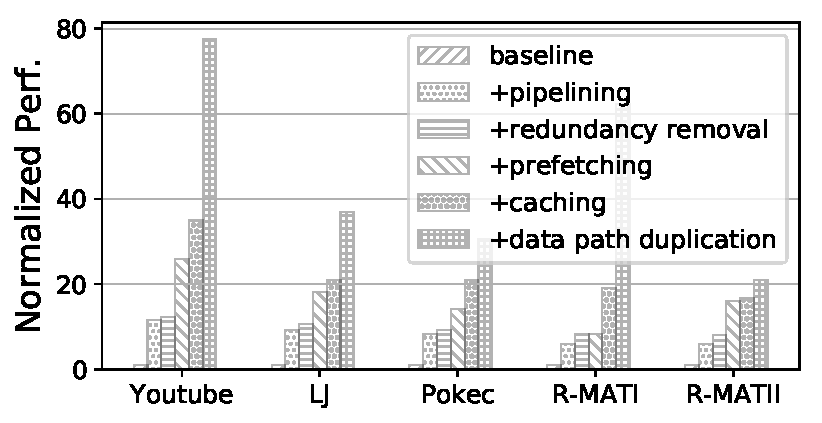
\includegraphics[width=0.95\linewidth]{opt-performance}}
    \caption{BFS accelerator optimization techqniue evaluation. The performance on 
    all the graphs improves when more optimizations including pipelining, 
    redundancy removal, prefetching, caching, and data path duplication are 
    gradually applied to the design.}
\label{fig:opt-performance}
\end{figure}

\section{Conclusions} \label{sec:conclusion}
Handcrafted HDL based BFS accelerators usually suffer high portability and maintenance cost 
as well as ease of use problem despite the relatively 
good performance. HLS based BFS accelerator can greatly alleviate these problems, but it is 
difficult to achieve satisfactory performance due to the inherent irregular memory access and 
complex nested loop structure. In this work, we stream the basic BFS algorithm and develop 
a series of HLS based optimizations such as redundancy removal, prefetching, caching and 
data path duplication. According to the experiments on 
a representative graph benchmark, the resulting HLS based BFS accelerator achieves up to 70X speedup 
compared to a baseline HLS design with best-effort HLS pragma optimization. When compared to the 
existing HDL based BFS accelerators on similar FPGA cards, the proposed HLS based BFS accelerator 
gets around 35\% of the MTEPS, but it preserves the nice software-like features including 
portability and ease of use and maintenance, and achieves higher per bandwidth MTEPS in some cases 
mostly because of the graph specific optimization techniques. 

